\subsection{Postoperativt}
Udover præoperative faktorer kan der postoperative komplikationer som ikke kan tages højde for præoperativt, herunder komplikation påstået under og efter operation, som kan have indflydelse på en længere indlæggelsesvarighed for patienten. Postoperativ estimeres indlæggelsesvarigheden ligeledes ikke på nuværende tidspunkt, hvorfor der er taget udgangspunkt i informationspjecer fra ortopædkirurgisk afdeling på Aalborg Universitetshospital samt studier der påviser dette.

\subsubsection{Komplikation under operation}
Det fremgår af afsnit \ref{praeop} at demografiske-, livsstils- og kliniske faktorer kan have indflydelse på komplikationer under operationer. Dette kan bl.a. være blødning og selve operationstypen. De statistiske tests påviste at alder, rygning, diabetes og operationstype har en statistisk indflydelse på indlæggelsesvarigheden. Da flere af disse faktorer kan medføre komplikationer under operationen og længere operationsvarighed forventes det, at det i nogle tilfælde kan være mere omfattende operaioner, som kræver en længere operationsvarighed. Sammenhængen mellem operationsvarighed og indlæggelsesvarighed ses af \figref{opindlaeg}.


\begin{figure}[H]
	%\flushleft 
	\centering
	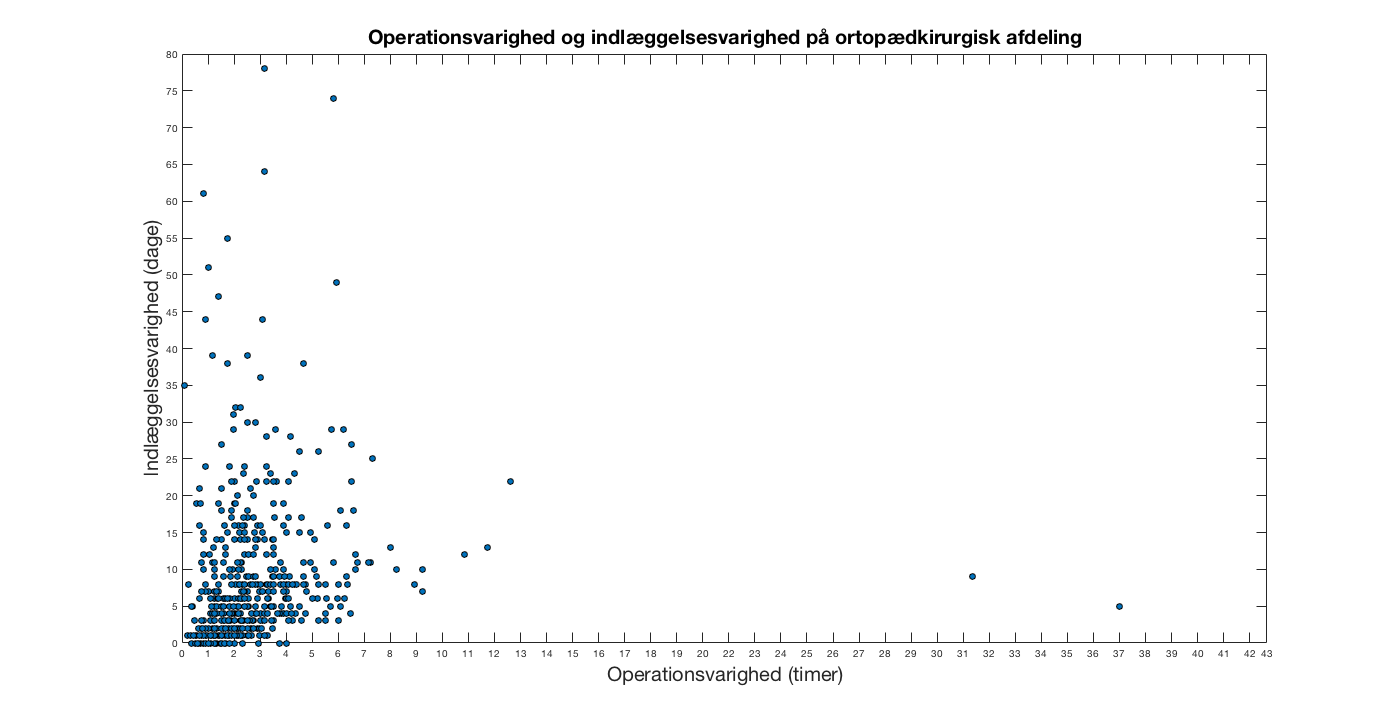
\includegraphics[scale=0.35]{figures/opindlaeg.png}
	%\flushleft
	\caption{\textit{Operationsvarighed og indlæggelsesvarighed for patienter på ortopædkirurgisk afdeling. Dette er over en periode på 3 måneder fra den 1. august til den 31. oktober år 2014.}}
	\label{opindlaeg}
	\end{figure}

\noindent
På \figref{opindlaeg} fremgår det, at operationerne på ortopædkirurgisk afdeling tager op til 37 timer, hvoraf de fleste operationer er centreret omkring 0 til 7 timer. Derudover ses det at to operationer ved hhv. 31,5 time og 37 timer varierer fra de resterende operationsvarigheder. Den gennemsnitlige indlæggelsesvarighed er for patienter på 9,25 dage, mens den gennemsnitlige operationstid er på 3 timer. 

For at undersøge om der er en statistisk sammenhæng mellem indlæggelsesvarigheden og operationsvarighed udføres en korrelationstest. Resultatet af denne test kan fremgår af \tabref{opogindlaegtab}.

\begin{table}[H]
\centering
\begin{tabular}{|c|c|c|}
\hline
\textbf{}                                             & \textbf{Sub-sample} & \textbf{P-værdi} \\ \hline
\textbf{Indlæggelsesvarighed ift. operationsvarighed} & 486                 & 0,016*           \\ \hline
\end{tabular}
\caption{Korrelationstest for sammenhæng mellem indlæggelsesvarigheden og operationsvarighed. P-værdier under et signifikantsniveau på 5\% er angivet med *.}
\label{opogindlaegtab}
\end{table}

\noindent
På \tabref{opindlaegtab} ses p-værdier for sammenhængen mellem indlæggelsesvarigheden og operationsvarigheden. Det fremgår, at der er en statistisk sammenhæng mellem indlæggelse- og operationsvarigheden. 

\subsubsection{Komplikationer efter operationen}
Det tyder på, at bevægelighed efter operation er vigtigt for, at komme sig hurtigt efter operationen, da dette er med til, at mindske risikoen for komplikationer og smerter efter operationen. Sammenhængen mellem træning og indlæggelsesvarigheden er illustreret på \figref{traeningindlaeg}.

\begin{figure}[H]
	%\flushleft 
	\centering
	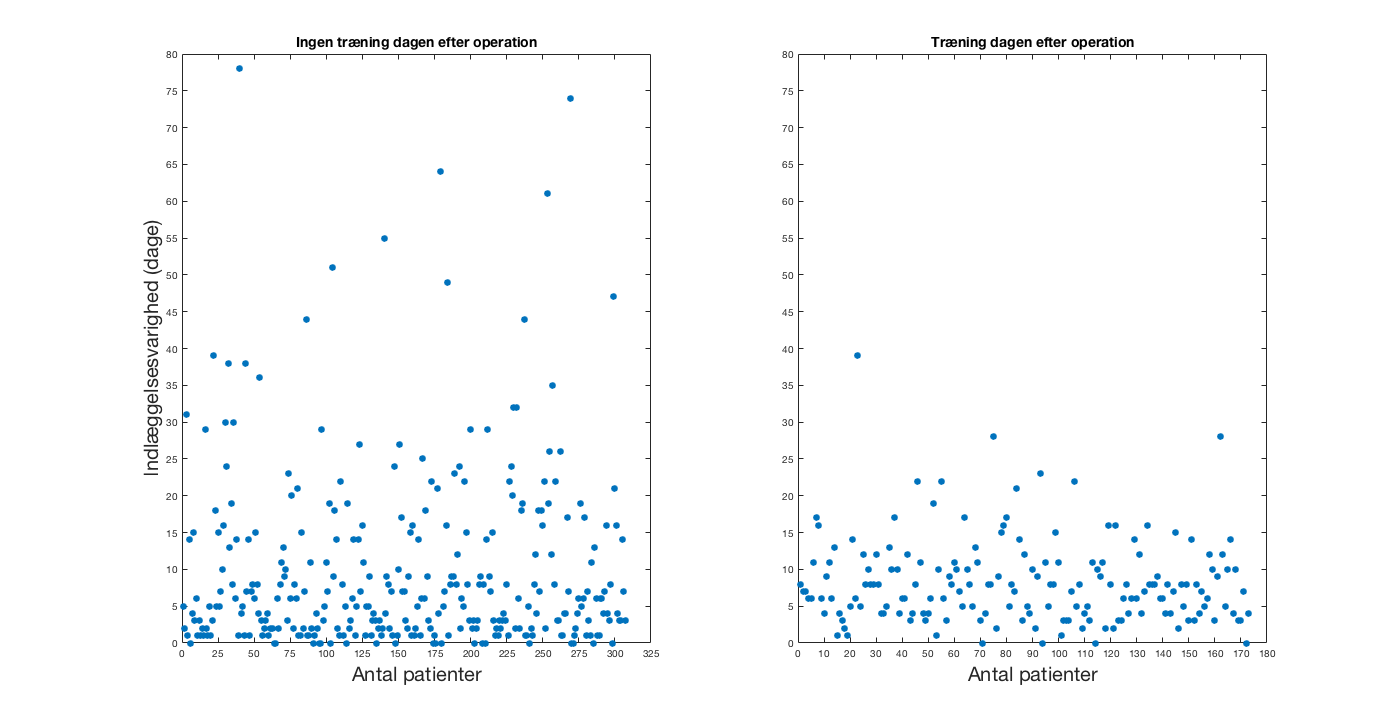
\includegraphics[scale=0.35]{figures/traeningindlaeg.png}
	%\flushleft
	\caption{\textit{Træning og indlæggelsesvarighed for patienter på ortopædkirurgisk afdeling. Træning er opdelt i ingen træning dagen efter operation og træning dagen efter operation. Dette er over en periode på 3 måneder fra den 1. august til den 31. oktober år 2014.}}
	\label{traeningindlaeg}
	\end{figure}

\noindent
På \figref{traeningindlaeg} fremgår det, at der er flere patienter  der ikke træner dagen efter operationen. Ligeledes er variationen i indlæggelsesvarighed større for patienter der ikke træner dagen efter end patienter der træner. Den gennemsnitlige indlæggelsesvarighed for patienter, der ikke træner dagen efter operation er 10 dage. Modsat er patienter, som træner dagen efter operationen 8,2 dage. Det tyder derfor på, at træning har en betydning for indlæggelsesvarigheden. 

For at teste om der signifikant sammenhæng mellem indlæggelsesvarighed og træning efter operationen udføres to sample t-test. Resultaterne heraf fremgår af \tabref{traeningindlaegtab}. 

\begin{table}[H]
\centering
\begin{tabular}{|c|c|c|c|}
\hline
\textbf{Træning}    & \textbf{Sub-sample} & \textbf{Indlæggelsesgennemsnit} & \textbf{P-værdi} \\ \hline
Ingen træning dagen efter operation      & 307                 & 9,95                            & 0,2248           \\ \hline
Træning dagen efter operation & 173                 & 8,24                            & 0,0950*          \\ \hline
\end{tabular}
\caption{Statistik over sammenhæng mellem indlæggelsesvarigheden og træning dagen efter operation. P-værdier under et signifikantsniveau på 5\% er angivet med *.}
\label{traeningindlaegtab}
\end{table}

\noident 
På \tabref{traeningindlaegtab} fremgår p-værdier for sammenhængen mellem indlæggelsesvarigheden og træning dagen efter operationen. Det ses at der er en statistisk sammenhæng mellem indlæggelsesvarigheden og træning dagen efter operation. Patienter der træner dagen efter operationen er i gennemsnit indlagt kortere tid end den gennemsnitlige patient. Det tyder der på, at træning har en indflydelse på indlæggelsesvarigheden. 


\subsubsection{Udskrivelse af patienter}
Foruden komplikationer opstået under operationen samt efterfølgende kan afhentning af patienterne have indflydelse på en forlænget indlæggelsesvarighed grundet udskrivningen af patienter. I nogle tilfælde kan patienter, der er klar til at blive udskrevet være nødsaget til at ligge en dag ekstra på afdelingen, da de har brug for pleje i hjemmet efter operationen. Hvis det er nødvendigt med hjemmepleje kræver det, at afdelingen kontakter kommunen før kl. 12 samme dag. Hvis personalet ikke når dette skal patienten blive på afdelingen endnu et døgn. 

Derudover kan nogle patienter, der skal have efterbehandling eller genoptræning,  nødsaget til at blive på afdelingen, da deres hjem ikke er tilpasset til dette. 

Dette kan også gælde patienter, som i forvejen har komorbiditeter, hvor forandringer grundet operationen og indlæggelsen forværrer deres tilstand. Dette kan eksempelvis være demens, hvor patienten mister evnen til at varetage sit eget helbred. Disse patienter skal ofte vente på at der er en aflastningsplads ledig før disse kan udskrives fra afdelingen. 


